\documentclass{article}      % arxiv.sty sets its own 10pt-based font sizes

\usepackage{arxiv}          % arxiv-style preprint template (paper/arxiv.sty)

\usepackage[utf8]{inputenc} % allow utf-8 input
\usepackage[T1]{fontenc}    % use 8-bit T1 fonts
\usepackage{hyperref}       % hyperlinks
\usepackage{url}            % simple URL typesetting
\usepackage{booktabs}       % professional-quality tables
\usepackage{amsmath}
\usepackage{amsfonts}       % blackboard math symbols
\usepackage{amssymb}
\usepackage{bm}
\usepackage{nicefrac}       % compact symbols for 1/2, etc.
\usepackage{microtype}      % microtypography
\usepackage{graphicx}
\usepackage{listings}
\usepackage{xcolor}

% --- Julia source-code listing style --------------------------------------
\definecolor{jlkw}{RGB}{130,60,150}
\definecolor{jlstr}{RGB}{170,60,40}
\definecolor{jlcom}{RGB}{110,110,110}
\lstdefinelanguage{Julia}{
  keywords={function,struct,mutable,end,for,while,if,else,elseif,return,using,
            import,module,export,const,where,in,begin,let,do},
  sensitive=true,
  morecomment=[l]{\#},
  morestring=[b]",
}
\lstset{
  language=Julia,
  basicstyle=\ttfamily\footnotesize,
  keywordstyle=\color{jlkw}\bfseries,
  stringstyle=\color{jlstr},
  commentstyle=\color{jlcom}\itshape,
  showstringspaces=false,
  columns=fullflexible,
  breaklines=true,
  frame=single,
  framerule=0.3pt,
  rulecolor=\color{gray!40},
}

\newcommand{\JuliaMag}{\textsc{JuliaMag}}
\newcommand{\mumax}{\textsc{mumax}$^3$}
\newcommand{\oommf}{\textsc{OOMMF}}
\newcommand{\vm}{\bm{m}}
\newcommand{\vB}{\bm{B}}

\title{\JuliaMag: a minimalist, dispatch-based micromagnetic solver in pure Julia}

% Short title for the running head (arxiv.sty puts \shorttitle in the header;
% by default it is the full \@title, which is too long).
\renewcommand{\shorttitle}{\JuliaMag}

\author{%
  R.~L.~Novak \\
  Universidade Federal de Santa Catarina (UFSC) -- Campus Blumenau \\
  Rua Marechal Rondon 880, 89065-200, Blumenau, Brazil \\
  \texttt{rafael.novak@ufsc.br}
}

\date{\today}

\begin{document}

\maketitle

\begin{abstract}
We present \JuliaMag, an open-source micromagnetic simulation package written
entirely in the Julia programming language. \JuliaMag{} solves the
Landau--Lifshitz--Gilbert (LLG) equation on a finite-difference mesh, including
the exchange, magnetostatic (demagnetizing), uniaxial anisotropy, Zeeman, and
Dzyaloshinskii--Moriya interactions, as well as the Zhang--Li and Slonczewski
spin-transfer torques. The code is designed around Julia's multiple dispatch:
every field and torque operates on an abstract array type, so the same source
runs unchanged on CPU and GPU arrays, and material parameters are read through
accessors so that a single-material and a multi-region (multilayer) simulation
share one implementation with no overhead in the uniform case. We describe the
data layout, the field and torque implementations, the FFT-accelerated
demagnetization convolution, the time integration and energy minimization, the
geometry/region model, the output and simulation interface, and a CUDA package
extension that adds GPU methods additively through dispatch. We validate
\JuliaMag{} against the \mumax{} and \oommf{} reference codes on the $\mu$MAG
standard problems~2, 4, and~5 --- covering static equilibria and the
demagnetizing field, dynamic magnetization reversal, and current-driven
spin-transfer torque --- reproducing the references to within
$\sim 4\times10^{-3}$ in the spatially averaged magnetization.
\end{abstract}

\keywords{micromagnetics \and Landau--Lifshitz--Gilbert equation \and
  finite-difference method \and Julia \and multiple dispatch \and GPU computing}

% ==========================================================================
\section{Introduction}
\label{sec:intro}

Micromagnetics is the continuum theory of ferromagnetic materials at the
sub-micron scale, in which the magnetization is treated as a continuous
vector field whose evolution is governed by the Landau--Lifshitz--Gilbert (LLG)
equation~\cite{miltat2007,abert2019}. Because the effective field entering the
LLG equation couples every part of the sample through the long-ranged
magnetostatic interaction, and because the exchange interaction imposes a short
length scale, analytical solutions exist only for the simplest geometries.
Numerical micromagnetics has therefore become an indispensable tool, from the
earliest finite-difference computations of domain-wall structure~\cite{labonte1969}
and the stochastic foundations of thermally activated
switching~\cite{brown1963} to today's routine simulation of spintronic devices,
skyrmions, and domain-wall memories.

Two finite-difference codes dominate the field. \oommf~\cite{oommf}, developed at
NIST, has been the community reference for over two decades. \mumax~\cite{mumax3}
brought micromagnetics to the graphics processing unit (GPU), achieving order-of-
magnitude speedups~\cite{lopezdiaz2012} and enabling simulations that were
previously impractical. Both are highly optimized, but both are also large,
performance-tuned codebases --- \oommf{} in C\texttt{++} with a Tcl interface,
\mumax{} in Go with hand-written CUDA kernels --- in which the numerical methods
are interwoven with low-level implementation detail. For a researcher who wishes
to read, modify, or extend the core algorithms, or to prototype a new physical
term or solver, this coupling is a barrier.

The central computational cost in both codes is the magnetostatic
(demagnetizing) field, a dense convolution of the magnetization with a geometric
kernel. Evaluated directly it scales as $O(N^2)$ in the number of cells; the
standard remedy, adopted here, is the fast-Fourier-transform convolution of
Hayashi \textit{et al.}~\cite{hayashi1996}, which reduces the cost to
$O(N\log N)$ and remains the workhorse of finite-difference
micromagnetics~\cite{lepadatu2019}.

We present \JuliaMag, a micromagnetic solver written entirely in the Julia
programming language~\cite{julia}. Our aim is not to outperform the established
GPU codes but to provide a \emph{transparent} and \emph{extensible} reference
implementation in which the numerical methods are expressed directly, at the
level of the mathematics, and are validated against \oommf{} and \mumax{} to high
accuracy. Julia is well suited to this goal: it combines a high-level,
mathematical syntax with performance approaching that of C, and its multiple
dispatch lets a single generic implementation of each field and torque serve both
CPU and GPU arrays without duplication. The scientific Julia ecosystem, in
particular the \texttt{DifferentialEquations.jl} suite~\cite{diffeq}, further
supplies community-validated adaptive time integrators that we use directly in
place of a hand-rolled solver.

The remainder of the paper describes the theory (Sec.~\ref{sec:theory}), the
architecture and data layout (Sec.~\ref{sec:arch}), the effective-field terms and
the FFT-accelerated demagnetization (Sec.~\ref{sec:fields}), the torques
including spin-transfer (Sec.~\ref{sec:torques}), the time integration and energy
minimization (Sec.~\ref{sec:solvers}), the initial states and I/O
(Sec.~\ref{sec:config}), the geometry and material-region model
(Sec.~\ref{sec:regions}), the output and simulation interface
(Sec.~\ref{sec:interface}), and the GPU package extension
(Sec.~\ref{sec:gpu}). Section~\ref{sec:validation} validates \JuliaMag{}
against the \mumax{} and \oommf{} reference codes on the $\mu$MAG standard
problems~2, 4, and~5, which together exercise the static equilibria and
demagnetizing field, the dynamic magnetization reversal, and the spin-transfer
torque, respectively.

% ==========================================================================
\section{Theory}
\label{sec:theory}

The state of a micromagnetic system is the reduced magnetization field
$\vm(\bm{r},t) = \bm{M}(\bm{r},t)/M_s$, a unit-vector field with $M_s$ the
saturation magnetization. Its dynamics obey the Landau--Lifshitz--Gilbert (LLG)
equation, written here in the explicit (Landau--Lifshitz) form
%
\begin{equation}
  \frac{\partial \vm}{\partial t}
  = -\frac{\gamma}{1+\alpha^2}
    \Big[\, \vm\times\vB_{\mathrm{eff}}
          + \alpha\,\vm\times(\vm\times\vB_{\mathrm{eff}}) \,\Big],
  \label{eq:llg}
\end{equation}
%
where $\gamma$ is the gyromagnetic ratio and $\alpha$ the Gilbert damping. The
effective field $\vB_{\mathrm{eff}}$ is the variational derivative of the total
energy density $\varepsilon$ with respect to the magnetization,
%
\begin{equation}
  \vB_{\mathrm{eff}} = -\frac{1}{M_s}\frac{\delta \varepsilon}{\delta \vm},
  \label{eq:beff}
\end{equation}
%
a genuine field in tesla. It is the sum of the contributing terms,
%
\begin{equation}
  \vB_{\mathrm{eff}}
  = \vB_{\mathrm{exch}} + \vB_{\mathrm{demag}}
  + \vB_{\mathrm{anis}} + \vB_{\mathrm{DMI}} + \vB_{\mathrm{ext}},
  \label{eq:beffsum}
\end{equation}
%
each defined in Sec.~\ref{sec:fields}. Two current-driven spin-transfer torques,
of the Zhang--Li and Slonczewski types, are added to the right-hand side of
Eq.~\eqref{eq:llg} when a current is present (Sec.~\ref{sec:stt}).

We follow the convention of \mumax{}~\cite{mumax3} and \oommf{}~\cite{oommf}
throughout: the effective field carries no factor of $\mu_0$ in the exchange,
anisotropy, or DMI terms [Eq.~\eqref{eq:beff}]; $\mu_0$ appears only in the
demagnetizing and Zeeman fields, which are physical $\bm{B}$ fields.

% ==========================================================================
\section{Architecture}
\label{sec:arch}

\subsection{Design goals}

\JuliaMag{} is written to be \emph{minimal}, \emph{transparent}, and
\emph{portable to the GPU without a rewrite}. These goals are met by three
decisions that pervade the code.

\paragraph{Data layout.}
The magnetization is stored as a dense four-dimensional array of shape
$(3, N_x, N_y, N_z)$, with the Cartesian component as the fastest-varying index:
%
\begin{equation}
  \vm \;\longleftrightarrow\; \texttt{m::Array\{T,4\}}, \quad
  \vm(i,j,k) = \texttt{m[:,\,i,\,j,\,k]}.
\end{equation}
%
Placing the component first makes each cell's vector contiguous in memory, which
vectorizes the per-cell cross products and, crucially, lets the whole array map
onto a GPU \texttt{CuArray} without any restructuring. The element type \texttt{T}
is a type parameter, so a simulation runs in \texttt{Float64} on the CPU and in
\texttt{Float32} on the GPU with no change to the source.

\paragraph{Multiple dispatch.}
Every field and torque routine is written against the abstract signature
\texttt{AbstractArray\{T,4\}}:
%
\begin{lstlisting}
function exchange!(B::AbstractArray{T,4},
                   m::AbstractArray{T,4},
                   mesh, mat; add=false) where {T}
    # ... generic stencil ...
end
\end{lstlisting}
%
CPU execution passes an \texttt{Array}; GPU execution will pass a \texttt{CuArray}
and Julia dispatches to a device method with the same name. There are no
\texttt{if gpu} branches and no duplicated call sites; GPU support is additive.

\paragraph{Index convention.}
All routines use a single $(x,y,z)$, one-based index convention, and the
coordinate origin is placed at the geometric centre of the sample, so cell
centres run from $-L/2$ to $+L/2$ along each axis. This matches \mumax{} and lets
localized initial states (vortices, skyrmions) be positioned by translation
(Sec.~\ref{sec:config}).

\subsection{Package structure}

The package is organized as one module per physical concept:
\texttt{Mesh} and \texttt{Material} hold the geometry and parameters;
\texttt{magnetization}/\texttt{config} build states; \texttt{exchange},
\texttt{anisotropy}, \texttt{dmi}, \texttt{zeeman}, \texttt{demag\_kernel},
and \texttt{demag\_field} implement the effective-field terms;
\texttt{effective\_field} assembles them; \texttt{llg} and \texttt{stt} form the
torques; \texttt{solver}, \texttt{integrator}, and \texttt{minimizer} advance or
relax the state; \texttt{energy} computes energies; and \texttt{ovf} reads the
standard interchange format. The \texttt{World} type bundles a mesh, a material,
a cached demagnetization plan, and the applied field, and is the single object
passed to the dynamics.

% ==========================================================================
\section{Effective-field terms}
\label{sec:fields}

\subsection{Exchange}

In the continuum limit the Heisenberg exchange field is
%
\begin{equation}
  \vB_{\mathrm{exch}} = \frac{2A}{M_s}\,\nabla^2\vm,
  \label{eq:exch}
\end{equation}
%
with $A$ the exchange stiffness. The Laplacian is discretized with the standard
six-neighbour stencil,
$\nabla^2\vm|_c \approx \sum_{\text{axes}}(\vm_{-}+\vm_{+}-2\vm_c)/\Delta^2$.
At a free boundary a Neumann condition $\partial\vm/\partial n = 0$ is imposed by
taking the missing neighbour equal to the central cell, so its contribution
vanishes; across a periodic axis the index wraps around. We verified
Eq.~\eqref{eq:exch} against the analytic spin-wave field
$-\frac{2A}{M_s}q^2\vm$ for $\vm=(\sin qx,0,\cos qx)$ to a relative error of
$10^{-2}$ in the mesh interior.

\subsection{Uniaxial anisotropy}

For a uniaxial easy axis $\bm{u}$ and anisotropy constant $K_u$,
%
\begin{equation}
  \vB_{\mathrm{anis}} = \frac{2K_u}{M_s}(\vm\cdot\bm{u})\,\bm{u}.
  \label{eq:anis}
\end{equation}

\subsection{Dzyaloshinskii--Moriya interaction}

Two DMI forms are provided. The interfacial (N\'eel) DMI, for thin films with
broken inversion symmetry, has field
%
\begin{equation}
  \vB_{\mathrm{DMI}}^{\mathrm{int}}
  = \frac{2D}{M_s}
    \Big(\partial_x m_z,\ \partial_y m_z,\ -\partial_x m_x-\partial_y m_y\Big),
\end{equation}
%
with $D$ in J/m$^2$. The bulk (Bloch) DMI, for chiral B20 crystals, has
%
\begin{equation}
  \vB_{\mathrm{DMI}}^{\mathrm{bulk}} = -\frac{2D}{M_s}\,\nabla\times\vm,
\end{equation}
%
with $D$ in J/m$^3$. Gradients use central differences with the same Neumann /
periodic boundary treatment as the exchange field. We verified both forms term
by term against the corresponding \mumax{} kernels, and confirmed that a Bloch
helix seeded at the equilibrium period $L = 4\pi A/D$ has a smaller residual
torque than one at the wrong period.

\subsection{Demagnetizing field: kernel and FFT convolution}
\label{sec:demag}

The magnetostatic (demagnetizing) field is a convolution of the magnetization
with a mesh-dependent tensor $\hat{N}$,
%
\begin{equation}
  \vB_{\mathrm{demag}}(\bm{r})
  = \mu_0 M_s \sum_{\bm{r}'} \hat{K}(\bm{r}-\bm{r}')\cdot\vm(\bm{r}'),
  \label{eq:demagconv}
\end{equation}
%
where $\hat{K}$ (our stored kernel, equal to $-\hat{N}$) is the field of a
unit-magnetized source cell. Because $\hat{K}$ depends only on the cell offset,
it is computed once per mesh by adaptive brute-force integration of the
surface-charge field over each destination cell (the \mumax{} method): a cell is
sub-sampled more finely the closer it is to the source, and the source and
destination sub-grids are staggered to improve accuracy. Only the six independent
components of the symmetric tensor are stored.

Evaluating Eq.~\eqref{eq:demagconv} directly is $O(N^2)$ in the number of cells.
The convolution theorem reduces it to $O(N\log N)$: the magnetization is
zero-padded to a size that turns the circular FFT convolution into the linear
convolution required, the kernel is transformed once at setup, and each timestep
performs a forward real FFT, a pointwise tensor--vector product in Fourier space,
and an inverse FFT. The transformed kernel, the FFT plans, and the scratch
buffers are cached in a \texttt{DemagPlan} object built once per simulation. We
verified the FFT path against a direct real-space circular convolution with the
same kernel to a relative error of $10^{-8}$, an accuracy check independent of any
analytic approximation. The self-demagnetization factors of a cubic cell come out
to $1/3$ per axis and satisfy the trace sum rule $N_{xx}+N_{yy}+N_{zz}=1$.

% ==========================================================================
\section{Torques}
\label{sec:torques}

\subsection{Landau--Lifshitz torque}

The LLG torque [Eq.~\eqref{eq:llg}] is evaluated per cell as two cross products,
$\bm{p}=\vm\times\vB_{\mathrm{eff}}$ and $\bm{q}=\vm\times\bm{p}$, combined as
$-\frac{\gamma}{1+\alpha^2}(\bm{p}+\alpha\bm{q})$. Written over
\texttt{AbstractArray\{T,4\}}, the same routine serves CPU and GPU.

\subsection{Spin-transfer torques}
\label{sec:stt}

A spin-polarized current adds a torque to the right-hand side of
Eq.~\eqref{eq:llg}. \JuliaMag{} implements both standard forms, following the
\mumax{} kernels.

For an in-plane current through a magnetization texture, the Zhang--Li torque is
%
\begin{equation}
  \bm{\tau}_{\mathrm{ZL}}
  = \frac{-1}{1+\alpha^2}
    \Big[(1+\xi\alpha)\,\vm\times(\vm\times\bm{h}_s)
        + (\xi-\alpha)\,\vm\times\bm{h}_s\Big],
  \label{eq:zhangli}
\end{equation}
%
with adiabatic spin velocity $\bm{h}_s = (b\,\bm{J}\cdot\nabla)\vm$,
$b = \mu_B/[2\,e\,M_s(1+\xi^2)]$ (in \JuliaMag's convention, where $\gamma$ is
carried inside the torque), $\bm{J}=P\bm{j}$ the polarized current density, and
$\xi$ the non-adiabaticity. The gradient uses central differences with
Neumann/periodic boundaries.

For a perpendicular current in a spin valve, the Slonczewski torque is
%
\begin{align}
  \bm{\tau}_{\mathrm{SL}} &= g_\alpha\big[(A+\alpha B)\,\vm\times(\bm{p}\times\vm)
                             + (B-\alpha A)\,(\bm{p}\times\vm)\big], \\
  A &= \beta\,\epsilon,\quad B = \beta\,\epsilon',\quad
      g_\alpha = \frac{1}{1+\alpha^2}, \notag
\end{align}
%
with $\beta = (\hbar/e)\,j/(t\,M_s)$ (times $\gamma$ in our convention), fixed-layer
polarization direction $\bm{p}$, free-layer thickness $t$, angular efficiency
$\epsilon = P\Lambda^2/[(\Lambda^2+1)+(\Lambda^2-1)(\bm{p}\cdot\vm)]$, and the
secondary (field-like) term $\epsilon'$.

A subtlety worth recording: \mumax{} applies the gyromagnetic ratio $\gamma$ in
the time integrator (its step is $\gamma\,\Delta t$ times the torque), so its
torque kernels do \emph{not} contain $\gamma$. \JuliaMag{} instead carries
$\gamma$ inside the LLG torque; consequently the STT prefactors must be multiplied
by $\gamma$ to sit on the same scale. Omitting this factor leaves the
spin-transfer torque roughly $\gamma \sim 10^{11}$ times too small, and the
current has no visible effect --- a discrepancy we caught precisely because the
standard-problem-5 target below did not move.

% ==========================================================================
\section{Time integration and energy minimization}
\label{sec:solvers}

\JuliaMag{} advances Eq.~\eqref{eq:llg} in two complementary ways.

\paragraph{Time integration.}
For real-time dynamics we use the community-validated, adaptive Runge--Kutta
methods of \texttt{OrdinaryDiffEq.jl}, wrapping the LLG right-hand side as an
ordinary differential equation $\mathrm{d}\vm/\mathrm{d}t = f(\vm)$ with a
per-step callback that renormalizes $|\vm|=1$. The default method is
\texttt{Tsit5}, the modern fifth-order explicit Runge--Kutta that supersedes the
Dormand--Prince RK45 used by \mumax{}. A hand-rolled Dormand--Prince integrator is
retained for reference and passes an analytic Larmor-precession test exactly.

\paragraph{Energy minimization.}
Relaxing to equilibrium by integrating the damped LLG in time is impractical: the
stiff exchange field drives the adaptive step to its floor, so reaching a
nanosecond-scale equilibrium would take of order $10^{12}$ steps. Following
\mumax{}, we relax instead with a dedicated energy minimizer --- a
Barzilai--Borwein steepest-descent method on the unit sphere. Each step moves the
magnetization along the damping torque $\bm{\tau}=-\vm\times(\vm\times\vB)$ with an
exact Cayley rotation
$\vm' = [(4-\tau^2)\vm + 4\Delta t\,\bm{\tau}]/(4+\tau^2)$, $\tau^2=\Delta t^2|\bm{\tau}|^2$,
that preserves $|\vm|=1$ to machine precision. The step size $\Delta t$ is chosen
by the alternating Barzilai--Borwein formulas, and convergence is declared when
the recent per-cell displacement $\max\|\Delta\vm\|$ falls below a threshold. The
total energy of a relaxing film drops monotonically in the windowed sense (the
Barzilai--Borwein step is not strictly monotone step-to-step, as in \mumax{}),
providing an independent convergence check.

% ==========================================================================
\section{Initial states and I/O}
\label{sec:config}

Following \mumax{}, an initial state is a function \texttt{Config: (x,y,z) ->
vector} sampled at each cell centre. \JuliaMag{} provides uniform, vortex,
antivortex, vortex-wall, two-domain, random, and N\'eel- and Bloch-skyrmion
configurations. Localizable textures accept a circulation/charge and a core
polarity, and are placed anywhere with \texttt{translate}, mirroring \mumax's
\texttt{.Transl}. States are read from and written to OVF files (text and binary,
the standard micromagnetic interchange format), so a run can start from a saved
configuration and its snapshots can be visualized in OOMMF, \mumax, or ParaView,
or plotted directly as an out-of-plane colour map with an in-plane vector
overlay.

% ==========================================================================
\section{Geometry and material regions}
\label{sec:regions}

Non-trivial geometries and multi-material samples are built with the same
compositional, function-based style as the initial states. A \emph{shape} is a
predicate \texttt{Shape: (x,y,z) -> Bool}, true inside the sample, in centred
coordinates; primitives (cuboid, cylinder, ellipsoid, cone, superball, layer
slabs) combine through set operations (union, intersection, difference,
complement) and transforms (translate, scale, rotate). Painting a shape with an
integer identifier through \texttt{defregion!} assigns cells to material regions.

Material parameters are then either a single \texttt{Material} or a per-region
\texttt{RegionParams} carrying a lookup table for each parameter
($M_s$, $A$, $\alpha$, $K_u$, the DMI and spin-torque constants). This is where
Julia's multiple dispatch does structural work: every field routine reads its
parameters through accessors (\texttt{msat(params,i,j,k)}, \texttt{aex(...)},
\ldots). For a scalar \texttt{Material} the accessor ignores the cell index and
returns the constant, which the compiler inlines to a plain field read, so a
single-material simulation incurs \emph{no} lookup overhead; for a
\texttt{RegionParams} the same accessor indexes the region table. The field code
is written once and serves both. At a region interface the exchange coupling uses
the harmonic mean of the two stiffnesses (as in \mumax), and cells with
$M_s = 0$ represent unfilled geometry --- they source no field and, once the
magnetization there is cleared, feel no torque --- so a disc or a magnetic
multilayer is expressed by painting material into the desired shape. The
demagnetizing convolution weights each source cell by its own $M_s$, so a
multilayer with layer-dependent magnetization is handled correctly.

% ==========================================================================
\section{Output, materials, and the simulation interface}
\label{sec:interface}

The user selects what to tabulate from a library of quantities, following
\mumax's data-table model. Besides the time and the spatially averaged
magnetization (globally and per region), the table can record the total and
per-term energies, the maximum torque, the applied field, the topological charge,
and the tracked positions of a vortex core (peak $|m_z|$ with sub-cell
interpolation), a skyrmion (centroid of the topological-charge density), and a
domain wall (zero crossing of the averaged in-plane component). Rows are appended
on a chosen time interval.

A small library of standard materials (Permalloy, Fe, Co, Ni, CoFeB, YIG) returns
representative parameter sets by name. A \texttt{Simulation} object bundles the
geometry, parameters, magnetization, and output table so that a script mirrors
the \mumax{} workflow:
%
\begin{lstlisting}
sim = Simulation(mesh, material("Permalloy"))
setmag!(sim, VortexConfig(mesh))
savequantities!(sim, q_time(), q_m(),
                q_vortexcore(); every = 10e-12)
relax!(sim)
run!(sim, 1e-9)
writetable(sim.table, "out.txt")
\end{lstlisting}

% ==========================================================================
\section{GPU acceleration through multiple dispatch}
\label{sec:gpu}

The architectural payoff of the design appears at the GPU boundary. Because every
field, torque, and state operation is written against the abstract signature
\texttt{AbstractArray\{T,4\}}, and a CUDA device array \texttt{CuArray\{T,4\}} is
exactly such a type, GPU support is \emph{additive}: it requires neither a
rewrite of the physics nor any change to user code. Moving the magnetization to
the device with \texttt{togpu} causes every subsequent field and torque call to
dispatch, by the array type alone, to a GPU method --- there are no \texttt{if
gpu} branches and no duplicated call sites.

The GPU methods live in a Julia \emph{package extension} that loads only when
\texttt{CUDA.jl} is present, so the core package carries no GPU dependency. Each
method expresses the per-cell stencil with array programming --- shifted views
and fused broadcast --- rather than a hand-written scalar loop, so the same
expression compiles to a single GPU kernel on a \texttt{CuArray} and to
vectorized code on a host \texttt{Array}. The demagnetizing convolution reuses
the same FFT structure through \texttt{CUDA.CUFFT}. The element type \texttt{T} is
a type parameter throughout, so a device run in \texttt{Float32} follows from the
same source that runs in \texttt{Float64} on the CPU. This is the concrete sense
in which \JuliaMag{} ``explores'' Julia: multiple dispatch and parametric types
turn CPU/GPU portability and single/multi-material generality from code-
duplication problems into dispatch problems, resolved by the compiler.

% ==========================================================================
\section{Validation}
\label{sec:validation}

\subsection{Standard problem 2}
\label{sec:std2}

The $\mu$MAG standard problem~2~\cite{mumag2} tests static equilibrium states and
the demagnetizing field across a range of particle sizes. A rectangular prism of
aspect ratio $L:d:t = 5:1:0.1$ is saturated along the body diagonal $[1,1,1]$,
the field is removed, and the state is relaxed to remanence. The reduced size is
$d/\ell_{\mathrm{ex}}$, with the magnetostatic exchange length
$\ell_{\mathrm{ex}} = \sqrt{A/K_m}$ and $K_m = \tfrac12\mu_0 M_s^2$; for our
Permalloy parameters $\ell_{\mathrm{ex}} = 5.69$~nm. We relax each size with the
energy minimizer and record the remanent $\langle m_x\rangle$ (along the long
axis) and $\langle m_y\rangle$ (along $d$).

Figure~\ref{fig:std2} compares a sweep of sizes against the \oommf{} reference
table. The agreement tracks the reference across the whole range, from the small
single-domain limit ($\langle m_x\rangle\to 1$, $\langle m_y\rangle\to 0$) to the
large-particle flower state; for example, at $d/\ell_{\mathrm{ex}}=20$ we obtain
$(\langle m_x\rangle,\langle m_y\rangle)=(0.9702,0.0817)$ versus the reference
$(0.9701,0.0819)$. Standard problem~2 thus exercises the demagnetizing field and
the energy minimizer over a wide range of aspect-ratio-driven equilibria.

\begin{figure}[t]
  \centering
  
\includegraphics[width=\columnwidth]{figures/stdproblem2_compare.png}
  \caption{$\mu$MAG standard problem~2: remanent magnetization vs.\ reduced size
  $d/\ell_{\mathrm{ex}}$. \JuliaMag{} (markers) follows the \oommf{} reference
  (lines) from the single-domain limit to the flower state.}
  \label{fig:std2}
\end{figure}

The problem also specifies a hysteresis loop with the field applied along
$[1,1,1]$: the coercive field $H_c$ is the field at which the projection
$\vm\cdot[1,1,1]/\sqrt{3}$ vanishes, and the switching field $H_s$ marks the
irreversible reversal jump. We compute both by ramping the field down from
positive saturation and relaxing at each step with the energy minimizer.
Figure~\ref{fig:std2hyst} shows $H_c/M_s$ and $H_s/M_s$ against
$d/\ell_{\mathrm{ex}}$ overlaid on the \oommf{} reference; at
$d/\ell_{\mathrm{ex}}=5$, for instance, we obtain
$H_c/M_s = 0.0560$ and $H_s/M_s = 0.0570$ versus the reference $0.0561$ and
$0.0574$, the small $H_s$ offset set by the field-step resolution.

\begin{figure}[t]
  \centering
  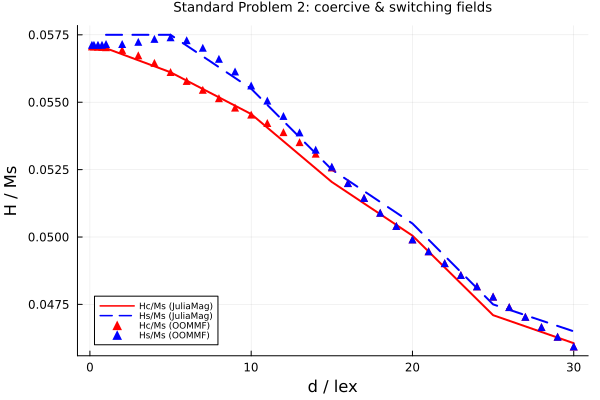
\includegraphics[width=\columnwidth]{figures/stdproblem2_hysteresis.png}
  \caption{$\mu$MAG standard problem~2: reduced coercive field $H_c/M_s$ and
  switching field $H_s/M_s$ vs.\ $d/\ell_{\mathrm{ex}}$. \JuliaMag{} (markers) vs.\
  the \oommf{} reference (lines).}
  \label{fig:std2hyst}
\end{figure}

\subsection{Standard problem 4}
\label{sec:std4}

The $\mu$MAG standard problem~4~\cite{mumag4} is the canonical test of dynamic
reversal. A $500\times125\times3$~nm Permalloy film ($M_s=8\times10^5$~A/m,
$A=1.3\times10^{-11}$~J/m, $\alpha=0.02$) is relaxed to its equilibrium S-state,
then field~1, $\mu_0\bm{H}=(-24.6, 4.3, 0)$~mT, is applied and the spatially
averaged magnetization $\langle\vm\rangle(t)$ is recorded for 1~ns. We relax the
S-state with the energy minimizer (375 steps) and integrate the switching with
\texttt{Tsit5}.

Figure~\ref{fig:std4} shows the result overlaid with \mumax{} and \oommf{}
reference runs. The three codes are visually coincident across the entire
nanosecond. Quantitatively, over $0$--$1$~ns the maximum deviation of
\JuliaMag{} from the references is
%
\begin{center}
\begin{tabular}{lccc}
\hline\hline
 & $\langle m_x\rangle$ & $\langle m_y\rangle$ & $\langle m_z\rangle$ \\
\hline
vs.\ \mumax{} & $0.0016$ & $0.0044$ & $0.0010$ \\
vs.\ \oommf{}  & $0.0037$ & $0.0035$ & $0.0011$ \\
\hline\hline
\end{tabular}
\end{center}
%
with root-mean-square deviations below $2\times10^{-3}$ for all components. The
relaxed S-state, $\langle\vm\rangle=(0.9668, 0.1256, 0)$, matches \mumax's
$(0.96697, 0.12528, 0)$.

\begin{figure}[t]
  \centering
  
\includegraphics[width=\columnwidth]{figures/stdproblem4_compare.png}
  \caption{$\mu$MAG standard problem~4: spatially averaged magnetization vs.\ time.
  \JuliaMag{} (solid lines), \mumax{} (circles), and \oommf{} (open triangles)
  coincide across the full nanosecond.}
  \label{fig:std4}
\end{figure}

\subsection{Standard problem 5}
\label{sec:std5}

The $\mu$MAG standard problem~5~\cite{najafi2009} tests the spin-transfer torque.
A $100\times100\times10$~nm Permalloy square ($M_s=8\times10^5$~A/m,
$A=1.3\times10^{-11}$~J/m) is relaxed to a vortex, then an in-plane current
$\bm{j}=(10^{12},0,0)$~A/m$^2$ with polarization $P=1$ and non-adiabaticity
$\xi=0.05$ is applied ($\alpha=0.1$). The current drives the vortex core to a
new equilibrium; the diagnostic is $\langle\vm\rangle$ at 1~ns.

We relax the vortex with the energy minimizer and integrate the current-driven
motion with a fixed-step fourth-order Runge--Kutta, adding the Zhang--Li torque
of Eq.~\eqref{eq:zhangli} to the LLG right-hand side. Starting from the centred
vortex, $\langle\vm\rangle=(0,0,0.027)$, the core migrates under the current and
settles at
%
\begin{equation}
  \langle\vm\rangle_{\JuliaMag}(1~\mathrm{ns}) = (-0.23488,\ -0.09453,\ 0.02296),
\end{equation}
%
against the \mumax{} reference $(-0.23480,\ -0.09454,\ 0.02296)$: a maximum
component deviation of $9\times10^{-5}$, within \mumax's own $10^{-4}$ tolerance.
Standard problem~5 thus validates the Zhang--Li spin-transfer torque
independently of the field terms exercised by standard problem~4.

% ==========================================================================
\section{Applications}
\label{sec:applications}

Beyond the quantitative benchmarks, two short studies illustrate the kind of
problem \JuliaMag{} is meant for: nonuniform equilibria on non-rectangular
geometry, and current-driven topological textures on a periodic wire. Both are
driven entirely through the user-facing simulation interface of
Section~\ref{sec:interface}.

\subsection{Vortex hysteresis in a disc}
\label{sec:vortex}

A magnetic vortex in a thin Permalloy disc traces a characteristic hysteresis
loop under an in-plane field~\cite{guslienko2002}. We take a
$500~\mathrm{nm}\times20~\mathrm{nm}$ disc, painted as a cylinder on a
$100\times100\times4$ mesh with the cells outside the disc left empty
($M_s=0$; Section~\ref{sec:regions}), and sweep the field along $x$ over
$\pm150$~mT, relaxing the magnetization with the energy minimizer at each step
and continuing from the previous state. Figure~\ref{fig:vortex} shows the result.
At zero field the centred vortex gives $\langle m_x\rangle=0$; the field displaces
the core along a nearly linear, reversible branch until, at the annihilation
field, the vortex is expelled and the disc jumps to its saturated branch
($\langle m_x\rangle\approx0.78$, below unity because shape demagnetization keeps
the edge spins curled). On the return branch the vortex renucleates, closing the
$S$-shaped loop. The disc must be wide and thin for the reversible
core-displacement branch to appear --- the signature that distinguishes a vortex
loop from a square one --- which is exactly the regime where an accurate
demagnetizing field matters most.

\begin{figure}[t]
  \centering
  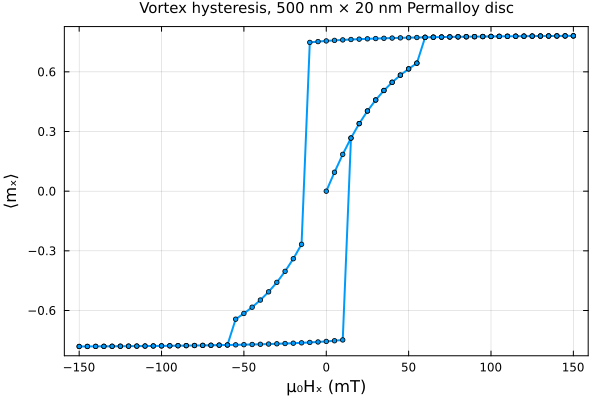
\includegraphics[width=\columnwidth]{figures/vortex_hysteresis.png}
  \caption{In-plane hysteresis loop of a magnetic vortex in a
  $500~\mathrm{nm}\times20~\mathrm{nm}$ Permalloy disc. The reversible
  core-displacement branch, the annihilation jump to the saturated branch, and
  the renucleation on the return sweep are all resolved.}
  \label{fig:vortex}
\end{figure}

\subsection{Current-driven skyrmion on an infinite wire}
\label{sec:skyrmion}

A N\'eel skyrmion stabilized by interfacial DMI and perpendicular anisotropy is
driven along a stripe by a Zhang--Li spin current. To model an infinite wire we
make the mesh periodic along $x$ ($\mathtt{pbc}=(1,0,0)$), so the skyrmion
re-enters from the far end rather than being pinned or annihilated at an edge; the
exchange, DMI, demagnetizing, and spin-torque terms all honour the periodic axis.
On a $300~\mathrm{nm}\times200~\mathrm{nm}\times1~\mathrm{nm}$ stripe
($M_s=5.8\times10^5$~A/m, $A=1.5\times10^{-11}$~J/m, $K_u=8\times10^5$~J/m$^3$,
$D=3.0\times10^{-3}$~J/m$^2$, $P=1$, $\xi=0.2$) a current
$\bm{j}=(2\times10^{12},0,0)$~A/m$^2$ drives the skyrmion against the electron
flow at a steady $v_x\approx-178$~m/s, with a transverse skyrmion-Hall deflection
along $y$. Figure~\ref{fig:skyrmion} shows the drift: the recorded position is
periodic, so it is unwrapped before fitting the velocity, giving a straight
$x(t)$ across the wrap-around re-entry, and the snapshots confirm the
hedgehog texture is preserved. The skyrmion position is obtained as the centroid
of the topological-charge density, computed circularly along the periodic axis so
that it remains correct when the texture straddles the wrap seam.

\begin{figure}[t]
  \centering
  
\includegraphics[width=\columnwidth]{figures/skyrmion_drive.png}
  \caption{Current-driven N\'eel skyrmion on a stripe made periodic along $x$
  (an infinite wire). (a)~Unwrapped longitudinal position $x(t)$; the slope gives
  $v_x\approx-178$~m/s. (b),(c)~$m_z$ colour maps at $t=0$ and $t=3$~ns: the
  skyrmion has drifted along $-x$ (re-entering through the periodic seam) and
  deflected along $+y$ by the skyrmion-Hall effect.}
  \label{fig:skyrmion}
\end{figure}

% ==========================================================================
\section{Conclusion and outlook}
\label{sec:conclusion}

We have presented \JuliaMag, a micromagnetic solver written entirely in Julia,
and shown that a transparent implementation --- one in which each field, torque,
and solver is expressed directly at the level of the underlying mathematics ---
can reproduce the established \oommf{} and \mumax{} reference codes to high
accuracy. On the $\mu$MAG standard problems the spatially averaged magnetization
agrees with the references to $\sim 4\times10^{-3}$ (dynamic reversal, standard
problem~4), to $\sim 10^{-3}$ in the remanence and coercive field across a wide
range of aspect ratios (static equilibria, standard problem~2), and to
$9\times10^{-5}$ for the current-driven vortex (spin-transfer torque, standard
problem~5). Beyond the benchmarks, the same interface handles a vortex hysteresis
loop on a non-rectangular disc and a current-driven skyrmion on a periodic
infinite wire (Section~\ref{sec:applications}). Three architectural choices carry
the design: a
component-first $(3,N_x,N_y,N_z)$ data layout, multiple dispatch on an abstract
array type, and a single $(x,y,z)$ index convention with the origin at the sample
centre. Together they keep the source small and, crucially, leave GPU support as
a purely additive step: because every routine already operates on
\texttt{AbstractArray\{T,4\}}, device execution requires only that the arrays be
\texttt{CuArray}s and that a handful of inner kernels acquire GPU methods, with no
change to the call sites --- the natural next stage of development, following the
path that took \mumax{} to the GPU~\cite{lopezdiaz2012}.

Beyond conventional acceleration, a transparent, dispatch-based, and fully
differentiable-by-construction Julia implementation is a natural substrate for
the machine-learning methods now reshaping computational micromagnetics. Two
directions are especially promising. First, the magnetostatic field --- the
dominant cost --- is increasingly being approximated or accelerated by neural
surrogates: physics-informed and physics-aware machine-learning schemes have been
applied to stray-field computation and to micromagnetic energy minimization,
replacing or preconditioning the expensive convolution and its associated
minimization~\cite{schaffer2023,schaffer2025,schaffer2022}. A minimizer and demag
solver expressed as ordinary Julia functions can be differentiated and composed
with such surrogates directly, without a foreign-function boundary. Second, the
LLG dynamics themselves can be learned or extrapolated: neural ordinary
differential equations have been used to forecast the outcome of spintronic
experiments~\cite{chen2022}, and the same \texttt{DifferentialEquations.jl}
ecosystem~\cite{diffeq} that supplies \JuliaMag's time integrator also provides
the adjoint-sensitivity and neural-ODE machinery on which such approaches are
built. Positioning \JuliaMag{} within this ecosystem --- rather than as an
isolated, hand-optimized binary --- is, in our view, its most significant
long-term advantage.

Immediate development priorities are the completion of GPU support, region-wise
material parameters and non-rectangular geometries, and finite-temperature
(stochastic) dynamics in the spirit of Brown~\cite{brown1963}. The code is open
source and available at \url{https://github.com/rlnovak/juliamag}.

\begin{acknowledgments}
\emph{[To be added by the author.]}
\end{acknowledgments}

\begin{thebibliography}{99}

% --- Reference codes ---
\bibitem{mumax3} A.\ Vansteenkiste, J.\ Leliaert, M.\ Dvornik, M.\ Helsen,
  F.\ Garcia-Sanchez, and B.\ Van Waeyenberge, ``The design and verification of
  MuMax3,'' AIP Adv.\ \textbf{4}, 107133 (2014).
  \url{https://doi.org/10.1063/1.4899186}.
\bibitem{oommf} M.\ J.\ Donahue and D.\ G.\ Porter, ``OOMMF User's Guide,
  Version 1.0,'' Interagency Report NISTIR 6376, National Institute of Standards
  and Technology, Gaithersburg, MD (1999).

% --- Numerical micromagnetics ---
\bibitem{miltat2007} J.\ E.\ Miltat and M.\ J.\ Donahue, ``Numerical
  Micromagnetics: Finite Difference Methods,'' in \textit{Handbook of Magnetism
  and Advanced Magnetic Materials}, edited by H.\ Kronm\"uller, S.\ Parkin,
  J.\ E.\ Miltat, and M.\ R.\ Scheinfein (Wiley, 2007).
  \url{https://doi.org/10.1002/9780470022184.hmm202}.
\bibitem{abert2019} C.\ Abert, ``Micromagnetics and spintronics: models and
  numerical methods,'' Eur.\ Phys.\ J.\ B \textbf{92}, 120 (2019).
  \url{https://doi.org/10.1140/epjb/e2019-90599-6}.
\bibitem{labonte1969} A.\ E.\ LaBonte, ``Two-Dimensional Bloch-Type Domain Walls
  in Ferromagnetic Films,'' J.\ Appl.\ Phys.\ \textbf{40}, 2450 (1969).
\bibitem{brown1963} W.\ F.\ Brown, Jr., ``Thermal Fluctuations of a Single-Domain
  Particle,'' Phys.\ Rev.\ \textbf{130}, 1677 (1963).
  \url{https://doi.org/10.1103/PhysRev.130.1677}.

% --- Demagnetizing field ---
\bibitem{hayashi1996} N.\ Hayashi, K.\ Saito, and Y.\ Nakatani, ``Calculation of
  Demagnetizing Field Distribution Based on Fast Fourier Transform of
  Convolution,'' Jpn.\ J.\ Appl.\ Phys.\ \textbf{35}, 6065 (1996).
\bibitem{lepadatu2019} S.\ Lepadatu, ``Efficient computation of demagnetizing
  fields for magnetic multilayers using multilayered convolution,'' J.\ Appl.\
  Phys.\ \textbf{126}, 103903 (2019). \url{https://doi.org/10.1063/1.5116754}.

% --- GPU micromagnetics ---
\bibitem{lopezdiaz2012} L.\ Lopez-Diaz, D.\ Aurelio, L.\ Torres, E.\ Martinez,
  M.\ A.\ Hernandez-Lopez, J.\ Gomez, O.\ Alejos, M.\ Carpentieri, G.\ Finocchio,
  and G.\ Consolo, ``Micromagnetic simulations using Graphics Processing Units,''
  J.\ Phys.\ D: Appl.\ Phys.\ \textbf{45}, 323001 (2012).
  \url{https://doi.org/10.1088/0022-3727/45/32/323001}.

% --- Standard problems ---
\bibitem{mumag2} $\mu$MAG Standard Problem~2,
  \url{https://www.ctcms.nist.gov/~rdm/std2/spec2.html}.
\bibitem{mumag4} $\mu$MAG Standard Problem~4,
  \url{https://www.ctcms.nist.gov/~rdm/std4/spec4.html}.
\bibitem{najafi2009} M.\ Najafi \textit{et al.}, ``Proposal for a standard
  problem for micromagnetic simulations including spin-transfer torque,''
  J.\ Appl.\ Phys.\ \textbf{105}, 113914 (2009).

% --- Magnetization textures ---
\bibitem{guslienko2002} K.\ Yu.\ Guslienko, V.\ Novosad, Y.\ Otani, H.\ Shima,
  and K.\ Fukamichi, ``Magnetization reversal due to vortex nucleation,
  displacement, and annihilation in submicron ferromagnetic dot arrays,''
  Phys.\ Rev.\ B \textbf{65}, 024414 (2001).
  \url{https://doi.org/10.1103/PhysRevB.65.024414}.

% --- Machine learning in micromagnetics (perspectives) ---
\bibitem{schaffer2023} S.\ Schaffer, T.\ Schrefl, H.\ Oezelt, A.\ Kovacs,
  L.\ Breth, N.\ J.\ Mauser, D.\ Suess, and L.\ Exl, ``Physics-informed machine
  learning and stray field computation with application to micromagnetic energy
  minimization,'' J.\ Magn.\ Magn.\ Mater.\ \textbf{576}, 170761 (2023).
  \url{https://doi.org/10.1016/j.jmmm.2023.170761}.
\bibitem{schaffer2025} S.\ Schaffer, T.\ Schrefl, H.\ Oezelt, N.\ J.\ Mauser, and
  L.\ Exl, ``Physics aware machine learning for micromagnetic energy
  minimization: Recent algorithmic developments,'' Comput.\ Phys.\ Commun.\
  \textbf{315}, 109719 (2025).
  \url{https://doi.org/10.1016/j.cpc.2025.109719}.
\bibitem{schaffer2022} S.\ Schaffer, N.\ J.\ Mauser, T.\ Schrefl, D.\ Suess, and
  L.\ Exl, ``Machine Learning Methods for the Prediction of Micromagnetic
  Magnetization Dynamics,'' IEEE Trans.\ Magn.\ \textbf{58}, 1 (2022).
  \url{https://doi.org/10.1109/TMAG.2021.3095251}.
\bibitem{chen2022} X.\ Chen, F.\ A.\ Araujo, M.\ Riou, \textit{et al.},
  ``Forecasting the outcome of spintronic experiments with Neural Ordinary
  Differential Equations,'' Nat.\ Commun.\ \textbf{13}, 1016 (2022).
  \url{https://doi.org/10.1038/s41467-022-28571-7}.

% --- Language / ecosystem ---
\bibitem{julia} J.\ Bezanson, A.\ Edelman, S.\ Karpinski, and V.\ B.\ Shah,
  ``Julia: A Fresh Approach to Numerical Computing,'' SIAM Rev.\ \textbf{59}, 65
  (2017).
\bibitem{diffeq} C.\ Rackauckas and Q.\ Nie, ``DifferentialEquations.jl -- A
  Performant and Feature-Rich Ecosystem for Solving Differential Equations in
  Julia,'' J.\ Open Res.\ Softw.\ \textbf{5}, 15 (2017).

\end{thebibliography}

\end{document}
